\documentclass[12pt]{scrartcl}
\usepackage{comment} % enables the use of multi-line comments (\ifx \fi) 
\usepackage[english]{babel}
\usepackage[table,xcdraw]{xcolor}
\usepackage{longtable}
\usepackage{multirow}
\usepackage{graphicx}
\usepackage{booktabs}% für Tabelle
\usepackage{longtable}% für Tabelle
\usepackage{listings}
\usepackage[bottom=3cm, right=2.5cm, left=2.5cm]{geometry}
\usepackage{float}
\usepackage{wrapfig}
\usepackage{amsmath}
\usepackage{subcaption}

\usepackage[onehalfspacing]{setspace}
\usepackage{url}
\usepackage{tabularx}
\usepackage{caption}
\usepackage{eurosym}
\usepackage{svg}
\usepackage{pdfpages}
\usepackage{wrapfig}
\usepackage{color}
\usepackage{scrlayer-scrpage}%
\usepackage[T1]{fontenc}% wichtig für Trennung von Wörtern mit Umlauten
\usepackage{microtype}% verbesserter Randausgleich
\setlength{\headheight}{21.4pt}
\usepackage{apacite}
\usepackage{natbib}
\usepackage{eurosym}
\usepackage{amsmath}
\usepackage{algorithm}
\usepackage{algorithmicx}
\usepackage{eucal}% Special characters
\usepackage{amssymb}% math alphabet
\usepackage[noend]{algpseudocode}
\usepackage[utf8]{inputenc}
\usepackage[scaled]{helvet}
\renewcommand{\familydefault}{\sfdefault}

%% 11pt + helvetica + ohne %%% Math %%%
\DeclareMathOperator{\EX}{\mathbb{E}}% expected value
\DeclareMathOperator*{\argmax}{argmax}
\DeclareMathOperator{\argmin}{\arg\!\min}
%%% Coding %%%
\colorlet{punct}{red!60!black}
\definecolor{background}{HTML}{EEEEEE}
\definecolor{delim}{RGB}{20,105,176}
\colorlet{numb}{magenta!60!black}

\lstdefinelanguage{json}{
    basicstyle=\normalfont\ttfamily,
    numbers=left,
    numberstyle=\scriptsize,
    stepnumber=1,
    numbersep=8pt,
    showstringspaces=false,
    breaklines=true,
    frame=lines,
    backgroundcolor=\color{background},
    literate=
     *{0}{{{\color{numb}0}}}{1}
      {1}{{{\color{numb}1}}}{1}
      {2}{{{\color{numb}2}}}{1}
      {3}{{{\color{numb}3}}}{1}
      {4}{{{\color{numb}4}}}{1}
      {5}{{{\color{numb}5}}}{1}
      {6}{{{\color{numb}6}}}{1}
      {7}{{{\color{numb}7}}}{1}
      {8}{{{\color{numb}8}}}{1}
      {9}{{{\color{numb}9}}}{1}
      {:}{{{\color{punct}{:}}}}{1}
      {,}{{{\color{punct}{,}}}}{1}
      {\{}{{{\color{delim}{\{}}}}{1}
      {\}}{{{\color{delim}{\}}}}}{1}
      {[}{{{\color{delim}{[}}}}{1}
      {]}{{{\color{delim}{]}}}}{1},
}

%Pseudo-code indent
\algdef{SE}[SUBALG]{Indent}{EndIndent}{}{\algorithmicend\ }%
\algtext*{Indent}
\algtext*{EndIndent}

%Pseudo-code indent
\algdef{SE}[SUBALG]{Indent}{EndIndent}{}{\algorithmicend\ }%
\algtext*{Indent}
\algtext*{EndIndent}


%%%% footer and header %%%%
\setlength{\parindent}{0em}
\setlength{\parskip}{2mm}
\pagestyle{scrheadings}%  S
\clearscrheadfoot% 
\automark{section}% 
\setheadwidth{text}%
\ihead{\textbf{\pagemark}}
\renewcommand{\sectionmark}[1]{\markright{\ #1}} 
\ohead{\rightmark}
\KOMAoptions{headsepline=0.5pt}%
\renewcommand{\labelenumii}{\theenumii}
\renewcommand{\theenumii}{\theenumi.\arabic{enumii}.}
%%%% \footer and header %%%%

% Funktion, um besser Anführungszeichen zu setzen.
% Einfach \anf{Wort oder Text}
\newcommand{\anf}[1]{\glqq#1\grqq}
\begin{document}

\begin{titlepage}
\newgeometry{top=1cm, left=3cm, right=3cm}
\begin{tabular}{lcr}
  \hspace{10cm} &
  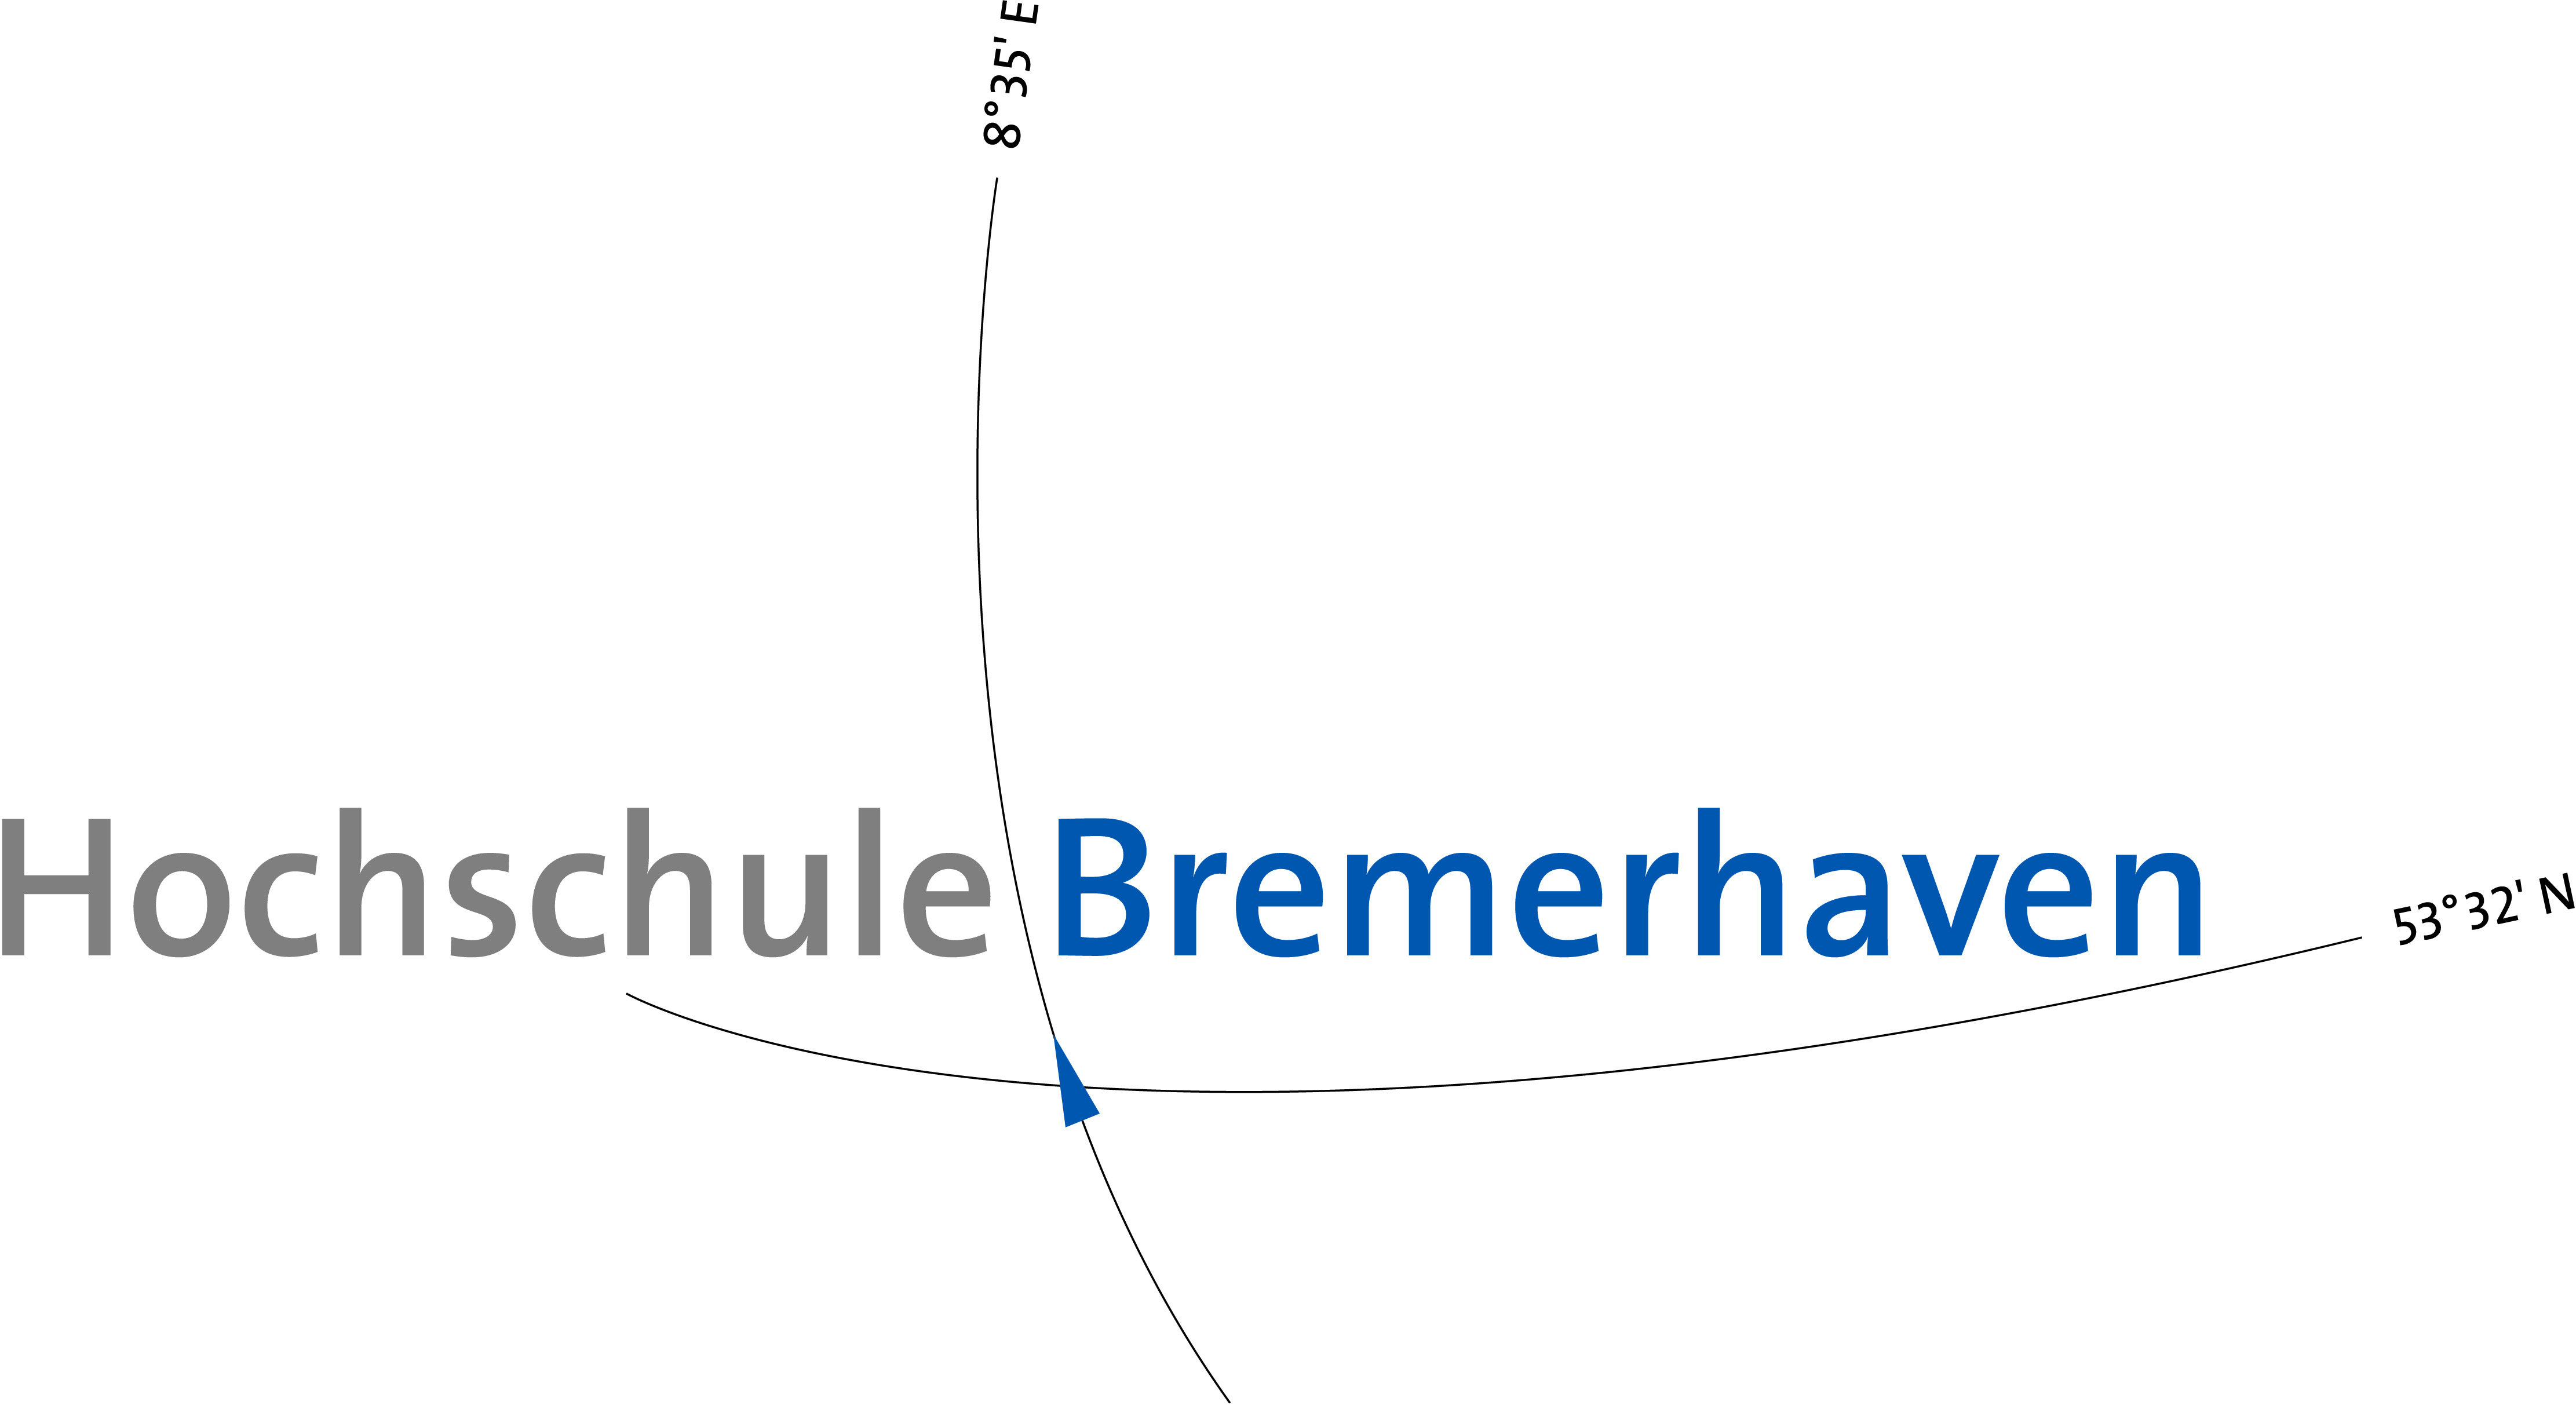
\includegraphics[width=170px]{images/hb_logo_2c.jpg}
  \vspace{1cm}
\end{tabular}
	\centering	
	\vspace{0cm}
	{\scshape\Large Digitalization, Innovation and Information Management \par}
	\vspace{1.5cm}
	{\Large\bfseries Master Thesis\par}
	\centering
    \vspace{2cm}
    {\Large\bfseries 
      Learning Representative Vessel Trajectories       Using  \par Deep Reinforcement Learning   \par
}
       {\normalsize\itshape
  Extracting Normality from AIS Data to Identify Anomalous Ship Behaviour
      \par}
	\vfill
	\vspace{2cm}
	\begin{tabularx}{\textwidth}{lX}
		Author: & Jan Löwenstrom (34937)\\
		Supervisors: & Prof. Dr.-Ing. Henrik Lipskoch \\ &(\textit{University of Applied Science Bremerhaven}) \\
		& Ph.D. Edgardo Solano Carrillo \\&(\textit{German Aerospace Center - Institute for the Protection of Maritime Infrastructures}, Bremerhaven)
		        
	\end{tabularx}  
    \vfill

% Bottom of the page with current date
	{\large \today \par}       
\end{titlepage}
\restoregeometry

% Inhaltsverzeichnis
\tableofcontents
\newpage

% Abbildungsverzeichnis
%\listoffigures
%\newpage
\noindent

\section{Prerequisites}
    \subsection{RL Framework}\label{chap:rlframework}
    In a reinforcement learning setup an agent is interacting with an environment $E$ at discrete time steps. At every time step $t$ the agent observes the current state of the environment $s_t$ and selects an action $a_t$. Feedback is returned by the environment in the form of a scalar reward $r_{t+1}$ and the resulting state $s_{t+1}$ based on the internal dynamics of the environment. We will use the definitions of \cite{Sutton1998} throughout this chapter, especially the definition of the point in time the reward is given back. In contrast to other publications like those from \cite{zare2021continuous}, \cite{wiering2012reinforcement} and \cite{lillicrap2019continuous}, \cite{Sutton1998} do not bind the reward signal to the same time step as the current state-action pair ($s_t$, $a_t$) but rather the next one, to indicate that the reward and the next state are calculated at the same time $t+1$.
This interaction can thus be illustrated in the following way, where the uppercase symbols $A$, $S$, and $R$ are used to indicate random variables. Their concrete instances of states, actions, or rewards are specified by the corresponding their lowercase symbols (e.g., $s_t$, $s_{t+1}$, or $a_t$):
\begin{figure}[H]
    \centering
    \hspace*{1cm}%
    \begin{tikzpicture}[]
\node (A) at (3,3) [rectangle, rounded corners, draw, minimum height=1cm,minimum width=3cm] {Environment};
\node (B) at (3,0) [rectangle, rounded corners, draw, minimum height=1cm,minimum width=3cm] {Agent};

\node (C) at (0.7, 3) [rectangle, thick, dashed, inner sep=0pt, minimum height=1cm, minimum width=0cm, draw] {};

\draw[->, black, very thick] ($(B.east)$) to[out=0,in=0, distance=2.5cm] ($(A.east)$);

\draw[->, black, very thick] ($(A.west)-(0.1,0)$)  to[out=3,in=7] ($(C.east) -(0,0.02)$);

\draw[->, black, very thick] ($(C.east) - (0,0.02)$) to[out=193,in=180, distance=2.4cm] ($(B.west)$);

\node[text width=3cm] at (1.6 , 4) 
    {$R_{t+1} S_{t+1}$};
    
\node[text width=3cm] at (-1.6 , 0.8) 
    {Observation \\ $S_t$};

\node[text width=3cm] at (-1.6, 2.2) 
    {Reward \\ $R_t$};
    
    
\node[text width=3cm] at (8.3, 1.5) 
    {Action \\ $A_t$};
    
\end{tikzpicture}
    \caption{Agent-environment interaction.}
    \label{fig:rlEnvironment}
\end{figure}



To be precise, we formalize the environment as a Markov decision process (MDP) with state space $\mathcal{S}$, continuous action space $\mathcal{A}$ , the transition dynamics $p(s_{t+1} \mid s_t, a_t)$ and reward function $r(s_t, a_t)$. The reward function is hand-crafted and indicates whether the selected action in a certain state is considered "good" or "bad". The action selection process or rather the \textit{behavior} of the agent is defined by a policy $\pi$, which is essentially a mapping from states to probabilities of actions being chosen $\pi: S \rightarrow P(A)$. But as we will exclusively calculate deterministic policies in this thesis, we define $\pi: S \rightarrow A$.
\newpage
One of the major challenges arises from the nature of an MDP being a sequential decision problem. An action that seems to be mediocre in the present may result in a trajectory that produces better rewards in the long run and vice versa. It is therefore necessary to take future rewards into account. The discounted sum of future rewards is called the \textit{return} with a discounting factor $\gamma \in (0,1]$  \cite[p.55]{Sutton1998}:

\begin{equation}\label{eq:discountedReturn}
    G_t = R_{t+1} + \gamma R_{t+2} + \gamma^2 R_{t+3} + \dots  = \sum_{k=0}^\infty{\gamma^k R_{t+k+1}}
\end{equation}

By reshaping the above equation, we can discover the relationship between consecutive returns \cite[p.55]{Sutton1998}:
\begin{equation}\label{eq:successiveReturn}
    \begin{aligned}
    G_t &= R_{t+1} + \gamma R_{t+2} + \gamma^2 R_{t+3} + \gamma^3 R_{t+4} + \dots \\
    &= R_{t+1} + \gamma (R_{t+2} + \gamma R_{t+3} + \gamma^2 R_{t+4} + \dots)  \\
   & = R_{t+1} + \gamma G_{t+1}
    \end{aligned}
\end{equation}

The overall objective of a reinforcement learning agent is therefore to find an optimal policy that maximizes the return for a given starting state $s_0$. In order to do so, reinforcement learning algorithms estimate the expected return for any given state or state-action pair, which is also called the \textit{value} or $Q$-value. The recursive relationship revealed in equation \ref{eq:successiveReturn} naturally applies to $Q$-values as well, which is formally described by the \textit{Bellman equation} (for discrete policies):

\begin{equation}
    Q^\pi(s_t, a_t) = \EX_\pi[r(s_t, a_t) + \gamma Q^\pi(s_{t+1}, \pi(s_{t+1})]
\end{equation}

Unfortunately, it is impossible to solve this equation if the model of the environment is unknown. Even if a perfect model is present, methods like \textit{Dynamic Programming} have limited utility due to their great computational expense \cite[p.~73]{Sutton1998}. Therefore, reinforcement learning algorithms take an iterative approach by interacting with the environment, sampling feedback and consecutively updating estimates of the actual returns. The closer those estimates are to the real values, the better the derived policy because the greediest policy will just select the action with the highest $Q$-value for every state.
\par
Tabular methods, as the name suggests,  keep all state-action pairs and their corresponding $Q$-value in big tables, updating them if needed. In contrast, deep reinforcement learning techniques utilize powerful function approximators like neuronal networks for the purpose of replacing the memory-limited tables and handling huge state and action spaces.
    \subsection{Neuronal Networks and PyTorch}
\section{Understanding Deep DPG}
The goal of this chapter is to dive deep into an actor-critic algorithm to build up in-depth knowledge about every aspect of this reinforcement learning approach. As \cite{tim2018} pointed out, this is a necessary step towards actually using those methods to their full potential because in case of a failure the researcher has intimate understanding and can bring up ideas on how to tweak certain aspects around the whole learning setup.
\par
To achieve said objective, we will take a very close look at an algorithm called \textit{Deep Deterministic Policy Gradient} (DDPG). Every element of this algorithm has its own sub-chapter where slices of the pseudo code from the original DDPG paper, published by \cite{lillicrap2019continuous}, will be included and discussed.


    \subsection{Actor-Critic Architecture}
    Recalling from the related work chapter \ref{chap:relatedWork}, DDPG is an off-policy algorithm that combines the \textit{Deterministic Policy Gradient} algorithm first introduced by \cite{silver2014deterministic} with the stability mechanisms of Deep Q-Learning (DQN). One major advantage of DDPG being a policy gradient method is the fact that it is able to handle problems with continuous action spaces  \cite[p.3]{lillicrap2019continuous} whereas DQN is limited to the discrete cases. This limitation arises due to the calculation of "best" actions given by the greedy policy $\max\limits_{a} Q(s_{t+1},a)$ which - for a discrete action space - is trivial. The Q-Learning algorithm just uses the expected return of the next state by simply selecting the one action in the set of actions that results in the highest consecutive Q-value. For the continuous case however, (Deep) Q-Learning would require an optimization of $a_t$ at every timestep to find the greedy policy which according to \cite{lillicrap2019continuous} "is too slow to be practical with large, unconstrained function approximators and nontrivial action spaces" (p.3).
\par
To overcome this challenge, policy gradient methods are conceptually different to action-value methods such as Q-Learning. Instead of learning action-values and using those estimates to derive a policy from, policy gradient methods maintain a function that can directly select actions without consulting a value function. This parameterized function $\mu_\theta(s)$ deterministically maps states to actions \cite[p.3]{lillicrap2019continuous} and represents the first component of the architecture - the \textit{actor}.
\par 
The actor adjusts the parameters $\theta$ of the policy in the direction of the performance gradient \cite[p.~2]{silver2014deterministic}. DDPG is an off-policy algorithm, which means that the ever-improving policy (target policy) is different from the one that interacts with the environment and gathers experience (behavior policy $\beta$). Therefore the off-policy deterministic policy gradient is defined and proven by \cite{silver2014deterministic} to be (p.~5): 
%\begin{equation}
%\begin{aligned}
 %   \nabla_{\theta^\mu}J &\approx \EX_{s_t \sim p^\beta}[
  %  \nabla_{\theta^\mu} Q(s,a\!\mid\! \theta^Q)\!\mid\! s\!=\!s_t, a\!=\!\mu(s_t\!\mid\!\theta^\mu)
 %   ] \\
 %   &= \EX_{s_t \sim p^\beta}[
 %   \nabla_a Q(s,a \!\mid\! \theta^Q) \!\mid\! s\!=\!s_t, %a\!=\!\mu(s_t) \nabla_{\theta_\mu} \mu(s \!\mid\! %\theta^\mu) \!\mid\! s\!=\!s_t]
 %   \end{aligned}
%\end{equation}

\begin{equation}\label{eq:policyGradient}
    \nabla_\theta J_\beta (\mu_\theta) = 
    \EX_{s \sim p^\beta}
    \Big[ \nabla_\theta \mu_\theta(s) \; \nabla_a Q^\mu (s,a) \!\mid_{a = \mu_\theta (s)} \! \Big]
\end{equation}


As we can see in equation \ref{eq:policyGradient}, the performance gradient not only depends on gradient of the policy with respect to the policy parameters but also on the true action-values $Q^\mu(s,a)$ with respect to the actions for the current actor policy $\mu$. Since the true action-values are unknown, a differentiable function $Q^ \omega(s,a)$ replaces $Q^\mu(s,a)$ in order to estimate those values. This estimation is done off-policy from trajectories generated by $\beta(a\!\mid\!s)$ using an appropriate policy evaluation algorithm like Temporal-Difference-Learning or Q-Learning \cite[p.~5]{silver2014deterministic}. $Q^ \omega(s,a)$ is also called the \textit{critic} and represents the second component of the actor-critic architecture. The word "critic" is used because $Q^ \omega(s,a)$ evaluates the returns for the current behaviour of the actor and simultaneously improves his performance because the actor ascends the gradient of the critic. Updating the critic is illustrated in the pseudo code by lines the 12 and 13. First, $y_i$ is defined as:
\begin{equation*}
    y_i = r_{i+1} + \gamma Q' (s_{i+1}, \mu'(s_{i+1} \mid \theta^{\mu'})  \mid \theta^{Q'})
\end{equation*}
to minimize the loss $L$, where $N$ is the batch size:
\begin{equation*}
    L = \frac{1}{N} \sum_i{(y_i - Q(s_i, a_i \mid \theta^Q))^2}
\end{equation*}
The actor update which is based on the off-policy deterministic policy gradient formalized in Eq. \ref{eq:policyGradient} can be found in line 15 of the pseudo code:

\begin{equation*}
                    \nabla_{\theta^\mu} J \approx \frac{1}{N}
                    \sum_i{\nabla_a Q(s, a \mid \theta^Q) 
                    \mid_{s = s_i, a=\mu(s_i)} \nabla_{\theta^\mu} \mu(s \mid \theta^\mu) \mid_{s_i}}
\end{equation*}
\par
DDPG utilizes neuronal networks as non-linear function approximators for the actor and critic. As mentioned earlier, the usage of those powerful approximators require additional modifications as convergence is no longer guaranteed \cite[p.3]{lillicrap2019continuous}. Those modifications include the two introductions of a replay buffer and a specific exploration noise which are discussed in detail in the next two sub-chapters but also the employment of mini-batches, batch-normalization and most perceptibly target networks. The target networks are essentially copies of the actor and critic networks ($\mu'_\theta(s)$ and $Q'^\mu(s,a)$) and their initial weight distributions. After each update to the actor and critic networks, a "soft" update is performed as well, which adjusts the weights of the target networks to a very small extent in the direction of the learned networks. This update procedure can be found in the pseudo code, where $\tau$ represents the update factor.
    \begin{equation*}
                    \theta^{Q'} \leftarrow \tau \theta^Q
 + (1- \tau) \theta^{Q'}                \end{equation*}
 \begin{equation*}
                    \theta^{\mu'} \leftarrow \tau \theta^\mu
 + (1- \tau) \theta^{\mu'}                
 \end{equation*}


\cite{lillicrap2019continuous} explain that "the target values are constrained to change slowly, greatly improving the stability of learning" and "that having both a target $\mu'$ and $Q'$ was \textit{required} to have stable targets in order to consistently train the critic without divergence" (p.~4).
    \subsection{Replay Buffer}
    The replay buffer is a finite size cache which stores transition tuples $(s_t, a_t, r_{t+1},s_{t+1})$ \cite[p.~4]{mnih2013playing}. Speaking in terms of programming, the replay buffer can just be an array of fixed-size $N$. After each interaction between agent and environment, another transition tuple is added to the array. If the array is filled up completely, the insert index gets reset to the first element, meaning that existing tuples are starting to get overwritten. It is worth noting that the replay buffer is not emptied throughout the learning process, so interactions over multiple episodes or even all past interactions can be present in the replay buffer at the same time. Each time the actor or critic is updated, a minibatch is randomly taken from the replay buffer to perform this update.
\par 
While conceptually simple, the notion of a replay buffer in the context of reinforcement learning is first introduced by \cite{lin1992reinforcement} to confront multiple challenges arising from the usage of neuronal networks in this domain. \cite{mnih2013playing} list three reasons why a replay buffer is better or rather inevitable for learning in conjunction with neuronal networks, in contrast to  the online variants.
\paragraph{Uncorrelated samples.} One of the most important  challenges emerges from the nature of the reinforcement learning setup and its sequential exploring.  Transition tuples get generated by the interaction between agent and environment step after step, resulting in highly correlated sequences of samples. Learning from those consecutive samples is inefficient because it would result in a high variance of updates \cite[p.~5]{mnih2013playing}. In this regard, \cite{lillicrap2019continuous} attest that "most optimization algorithms assume that the samples are independently and identically distributed" (p.~4) and that this assumption no longer holds if "samples are generated from exploring sequentially in an environment" (p.~4).
\par
It may sound counterproductive at first to learn from transition tuples that get selected completely at random. In the beginning, the replay buffer is filled with "bad" decisions of the past. Even if the agent explores a better state related to an improved action selection or the addition of noise, due to the fact that the replay buffer can easily contain hundreds of thousands of transitions, it may take a huge amount of learning steps until those new and desired transitions are even part of one mini-batch that passes the critic network once. But as the previous paragraph explained, the usage of a replay buffer is mandatory to break correlations between samples. Additionally, the concept of a pool to sample transitions from allows for the transformation of standard online Q-Learning to a more efficient variant because updates are based on batches instead of just the past interaction, which inherently results in higher data efficiency.

\paragraph{Data efficiency.} A single experience from the agent interaction with the environment is present in the replay buffer as long as it gets overridden. If the buffer is large enough and memory is no issue, it is certainly possible that a transition tuple stays in the replay buffer for the whole learning process. Consequently, this single piece of experience is potentially used in multiple weight updates, which results in higher data efficiency.

\paragraph{Avoiding feedback loops.} The third reason given by \cite{mnih2013playing} is an argument that endorses off-policy learning, like Q-Learning. They argue that on-policy learning will produce unwanted feedback loops or that parameters could get stuck in a poor local minimum (p.~5). 
\par 
The term on-policy is used when only one policy and its current parameters determine the next data sample, which is used to update exactly those parameters in return. On-policy methods do not make use of a separate behavior policy. This ultimately results in a  binding between the maximizing action and the training distribution. A replay buffer on the other hand averages the training distribution because it includes many past states. By smoothing out learning,
oscillations or divergence in the parameters can be avoided \cite[p.~5]{mnih2013playing}.
    \subsection{Exploration Noise}
    Adding a mechanism to any reinforcement learning algorithm that endorses the exploration of the state and action space is crucial in order to try many different decision paths and find a near optimal policy or \textit{the} optimal policy $\pi^*$. However, the policy that is constantly updated and improved during the learning process tries to fully exploit the environment as much as possible to collect the best returns that are currently know which can lead to the policy getting stuck in a local minimum. This contrast is also known as the exploration–exploitation dilemma \cite[p.~3]{Sutton1998}.
\par
The simplest and widely used approach in order to address this problem is the usage of an $\epsilon$-greedy policy, meaning that with probability $\epsilon$ a non-greedy action is taken \cite[p.~100]{Sutton1998}. Nevertheless this method is only suitable for discrete action where the policy selects from a set of actions. For the continuous case, some sort of noise has to be added to the suggested action value outputs of the actor. In the pseudo code, this is illustrated by the following line, where $\mathcal{N}$ is the component that generates the noise.
\par
\begin{equation*}
    a_t = \mu_\theta(s_t) + \mathcal{N}_t
\end{equation*}
\par 
The resulting value 
In the original DDPG Paper, \cite{lillicrap2019continuous} suggest the usage of a process that generates temporally correlated noise, specifically the Ornstein-Uhlenbeck process (OU process) \cite[]{uhlenbeck1930theory}. The authors justify their decision with the argument that this process very efficiently explores physical control problems with inertia (pp.~4,11). An OU process mainly depends on three variables. The mean of the noise $\mu$, the scale of the noise $\sigma$ and the rate of mean reversion $\theta$.
\par
//TODO
// generate plot of some theta and sigma combinations
\par
In later publications that try to improve certain aspects of the DDPG algorithm, it is mentioned that the utilization of the, to some extend complex, OU process is not needed and is in turn replaced by fixed Gaussian Noise. An example of this notion are \cite{fujimoto2018addressing} who state in their work about TD3 (an improved version of DDPG which addresses potential function approximation errors) that they "found noise drawn from the Ornstein-Uhlenbeck process offered no performance benefits" (p.~7). \cite{barth2018distributed} come to the same conclusion who describe that they "experimented with correlated noise drawn from an Ornstein-Uhlenbeck" but they "found this was unnecessary and did
not add to performance" (p.~5).
\par
Although we do not utilize a ship simulation and therefore the environment cannot be directly interpreted as physical problem, we still lay focus on the Ornstein-Uhlenbeck process as the main noise generator. The resulting ship trajectories from the AIS data still depend on the underlying ship dynamics even though they are part of a more abstract layer.
    \subsection{Hyper Parameters}
    In almost every machine learning scenario, the choice and search of suitable hyper parameters play an important role. The idea of this sub chapter is to give an overview of all relevant parameters, their description and some sort of default values or ranges that are mentioned numerous times in publications and programming frameworks. Furthermore 
\par
\paragraph{Discount factor $\boldsymbol{\gamma}$.} The discount factor describes how far the agent should factor future decisions and their rewards into its current decision. The author's previous bachelor thesis dealt intensively with the effects of this factor on the learning process. In summary, it can be said that a discount factor tailored to the learning scenario leads to significantly faster convergence rates in contrast to choosing a value close to 1 which results in the highest amount of training steps needed to find the optimal policy. However, since the real-world problems to which RL is applied are usually very complex and require the agent's maximum foresight, reduced learning times are usually foregone and a discount factor very close to 1 is chosen. For that reason, $\gamma = 0.99$ is used throughout all experiments.

\paragraph{Network architecture} For both, the actor and critic, a suitable network architecture as in the amount of hidden layers and the number of neurons in each of them have to be defined. \cite{lillicrap2019continuous} make use of a structure for both components which is a hidden layer with 400 neurons and a second hidden layer with 300 neurons (p.11). The same structure can be found in many applied works on DDPG, which at the same time operate in very different use cases, see for example //TODO works with DDPG.
//TODO Edgardo first principle book about ML

\paragraph{Learning rates} The learning rates of the actor and critic networks, $\alpha_\mu$ and $\alpha_Q$, determine
how much the model parameters should adjust to the calculated gradients in order to minimize the network's loss function. \cite{lillicrap2019continuous} utilize step sizes of $\alpha_\mu = 10^{-4}$ and $\alpha_Q = 10^{-3}$ (p.~11) without explicitly explaining why the critic changes faster than the actor. Regarding this topic, \cite{degris2012off} make the assumption that the setting of a slower updating actor in comparison to the critic is "desirable because we  effectively want
a converged value function estimate for the current
policy weights" (p.~5). This assumption also gets referenced in the original DPG paper \cite[p.~6]{silver2014deterministic}.
\par 
The ratio of the learning rates is kept in all experiments while trying out different scales of magnitude.

\paragraph{Batch size} For each training step, the batch size determines the amount of transition tuples are taking out of the replay buffer and fed through the neuronal networks in order to perform one network update. \cite{lillicrap2019continuous} perform update with a batch size of 64 (p.~11), whereas the RL library used in this thesis, Stable Baselines 3 (SB3), suggests a default parameter of 100. Overall we do not experience major variances in the outcomes when using different values for the batch sizes that are in the range of 32 to 256. 

\paragraph{Soft update parameter $\tau$} Tau determines how much the weights of the target networks should adjust to the direction of the learned networks. \cite{lillicrap2019continuous} use a value of $\tau = 0.001$ (p.~11), whereas SB3 suggests a default value of 0.005. //TODO

\paragraph{Noise parameter} The mean of the noise is defined to be 0 because the activation function of the final output layer of the actor is the hyperbolic tangent (also referred to as "tanh") which clips the suggested actions to the range of -1 to 1. The parameters $\sigma$ for the scale of the noise and $\theta$ for the rate of mean reversion can vary a lot depending on the amount of exploration needed for a specific environment. In our work, we keep $\theta$ more or less constant at 0.15 while just experimenting with different $\sigma$ values between 0.05 and 0.5. 
\section{Imitation Learning}
    In the previous chapter, we dove deep into a popular algorithm that is part of the classic approach of online RL. Sampling experience in the form of transition tuples by direct interactions with an environment, those methods do not require a predefined dataset. This greatly separates them from other machine learning disciplines like supervised or unsupervised learning.
\par 
In this chapter, we introduce the reader to a another approach of receiving an intelligent agent that has a very close relationship to reinforcement learning - \textit{Imitation Learning}. Foremost, we will discuss the major challenges and downsides of classic interactive online RL, followed by an exotic side trip into the fields of psychology and nature to then interpret the vessel path prediction problem from a different perspective. Afterwards, we take a closer look at a method called \textit{Behavioral Cloning}, followed by an investigation of an approach that reconstructs a hidden reward function based on expert demonstrations, to then use classic online RL algorithms such as DDPG to learn the underlying policy. 
        \subsection{Weaknesses of Interactive RL}
        Although directly interacting RL methods show great performance in a variety of different fields such as robotics and autonomous control \cite[]{etemad2020using, patil2021deep, wang2018reinforcement}, healthcare \cite[]{tseng2017deep, yu2019incorporating},  communication and networking \cite[]{chinchali2018cellular, fadlullah2017state}  or games \cite[]{berner2019dota, mnih2013playing, wu2016training}, they have got some weaknesses. One of them being the formulation of the most important component in order to successfully solve a task - the reward function. Designing a suitable reward signal by hand is a challenging but crucial job. Given, for example, a complex environment with long decisions trajectories until the terminal state - chess. If the reward is too sparse (feedback only at the very end of a game depending on the result), then the agent is likely to never explore a trajectory that results in winning the game and updating the state-action values accordingly. Contrary to that, a reward signal can be chosen so that it gives feedback in every state and almost explicitly tries to guide the agent. Such a reward function requires extensive task and domain knowledge but is also very subsceptible to the agent getting stuck in a local maximum. In the example of chess, this can be the assignment of a big positive reward when removing the opposing queen. Even though many players would agree, that getting rid of the enemy's queen is almost game winning, the agent might still not win a single game after that because it learns to just focus on removing the enemy's queen without having a strategy to actually win the game. Additionally, if the heuristic that determines the current board setting is defined by a human, the agent is bound to the human's view of playing the game which is manifested in the reward function. 
\par
Another weakness of RL methods that sample and learn directly from the interaction with an environment is the pure amount of interactions needed for the purpose of discovering a good-performing policy. In the literature, most algorithms are tested and benchmarked on classic control tasks (\textit{CartPole}, \textit{MountainCar}, \textit{Pendulum}, etc.), more challenging tasks (\textit{HalfCheetah}, \textit{Walker2d}, \textit{Humanoid}, etc.) in a physics engine such as \textit{MuJoCo} \cite[]{todorov2012mujoco} or take place in the field of game theory with examples such as the Atari games \cite[]{mnih2013playing}, Minecraft \cite[]{johnson2016malmo}, Starcraft 2 \cite[]{vinyals2019grandmaster} or Dota 2 \cite[]{berner2019dota}. Those environment as well as training environment in the context of robotics or autonomous control are either digital by nature or simulations of the real-word, which can be sped up and run in parallel during training. On top of that, failing (or rather discovering bad states) during the training phase has no real-world consequences like crashing a vehicle or hitting a wall or an obstacle with an remotely operated underwater vehicle (ROV) like the DLR-MI is using. Teaching an ROV to maneuver autonomously using interactive RL is impossible without a high-quality simulation.
\par
But even if a simulation with appropriate input and output interfaces is present, the complexity of the task can still demand huge amounts of computational power and millions of episodes. Good indicators for the complexity of a given task are the dimensions of the state and action spaces. We take the work from \cite{berner2019dota} as an extreme example as reference to our argument. They propose a system called "OpenAI five" which learns to play the popular and highly complex 5vs5 esports game "Dota 2" on such a high level that it is able to defeat the world champions of the year 2018. Without going into detail about the game itself, the agent has to interact with an environment that produces episodes of around 20,000 timesteps, an observation space of more than 16,000 states and a dynamic action space of 8,000 to 80,000 discrete actions \cite[p.~3]{berner2019dota}. To solve such a large problem in a way that it surpasses human performance is an impressive results, showing the potential of the reinforcement learning framework. However, the computing power and playtime required to discover such a policy far exceeds that of human learning to play the game. The system consists of over 1,000 GPUs and ~51,000 CPUs \cite[p.~3]{berner2019dota} and was trained on 45,000 years of Dota self-play over 10 realtime months \cite[]{OpenAI_dota}.
Numbers like this are more reminiscent of brute forcing than the ability to learn like a human, though it is most certainly impossible that a brute force method will ever be able to play Dota 2. \label{subchap:weak}
        \subsection{Nature as Blueprint}
        When we do write "learn like a human" as in the preceded subchapter, we refer to \textit{the} underlying motivation of reinforcement learning and the fact that it draws inspiration from psychological learning theories \cite[p.~341]{Sutton1998} and neuroscience \cite[p.~377]{Sutton1998}. Reinforcement learning is heavily influenced by the way humans and animals learn and interact with their real-world environment, based on for example chemical reward signals such as dopamine \cite[p.~383]{Sutton1998}. Taking nature or biology as blueprint to build artificial intelligence is not exclusive to the rl-framework. Neuronal networks for instance try to essentially copy the way our human brain works, with components even named "neurons" which are connected to each other (like synapses do in our brain) that reach different levels of activity (activation function).
\par
In our opinion it is a great advantage of reinforcement learning in general that it is so closely related to psychology and nature as a whole. It allows the researcher to take a step back from the formalism, algorithms and programming part in an effort to look at the problem from a different perspective. When we do take the example of playing Dota 2 from chapter \ref{subsec:weak}, there is a significant difference as to how we as human beings would approach such a task. One major advantage is the accumulated knowledge that we experienced in our prior lifespans. We do not start from zero, concepts like "enemies", "abilities" or "movement prediction" are already present that can be utilized and adopted in upcoming learning tasks. A whole research area focuses exactly on this ability, to learn from one task and transfer this knowledge to a different task - \textit{Transfer Learning} - which is out of scope for this thesis.
\par
Another great tool at our disposal is our talent to learn from others. In the case of Dota 2, these would be more experienced and better players that we face during our time playing the game. Our exceptional ability to mimic the behaviour of others (body movement, strategy, tool usage, etc.) might be inconspicuous to ourselves but is one key factor that we are able to solve new problems in relative short periods of time. It is also essential for the development of children as they usually start imitating their parents at an age of one to two \cite[p.347]{wood2013whom}. When trying to transfer this phenomenon from nature into the realm of machine learning, we find ourselves in an area summarized under the term \textit{Imitation Learning} (IL). It is the general approach of learning from an expert demonstrator in a supervised manner and sort of mimicking and generalizing its behaviour. Here, the demonstrator can either be a human expert that is familiar with the domain/task or an already trained artificial agent with a near optimal policy.
\par
RL and IL are very closely related, because they both try to solve problems that can be formulated as Markov Decision Processes and act within the same framework (see chapter \ref{chap:rlframework}). Additionally there even exist IL methods that actually utilize classic RL algorithms like DDPG after inversely reconstructing an underlying reward function (such a method is presented in chapter \ref{subchap:inverse}). What greatly separates IL from interactive RL methods is the fact that the reward function $r(s_t, a_t)$ does not have to be provided in the case of IL. As discussed in chapter $\ref{subchap:weak}$, the reward function is the most crucial component in order to tell the agent what desired goal it should reach. Nonetheless, this reward signal function is hand-crafted and can be hard to design especially if the researcher wants to "guide" the agent by utilizing non-sparse rewards that by some means defined sub-goals. (//TODO non-sparse rewards) IL in its simplest form drops the concept of reward functions entirely and makes the assumption that it is easier to demonstrate the desired behaviour than it is to specify the goal-oriented behaviour by a separate reward function as in RL. Therefore IL is also known as \textit{learning from demonstrations}. These demonstrations are recorded interactions from an expert with the environment $\tau = \{(s_t, a_t), (s_{t+1}, a_{t+1}), (s_{t+2}, a_{t+2}), \dots\}$ and are used to train a policy in a supervised manner that is way more efficient than classic interactive RL because trajectories of optimal behaviour are already given and do not have to be explored first.
\par
Although the upsides of IL (no hand-crafted reward function and very efficient policy learning) sound promising, it also has a major weakness in that in the naive approach violates the common "independent and identically distributed random variables" (i.i.d) assumptions made in statistical learning \cite{ross2011reduction} because the distributions of states encountered are different for the expert and trained agent. Intuitively this is because the train set overwhelmingly consists of "perfect" expert trajectories and if the agent makes just one mistake in a real rollout it will end up in a state that is totally unknown. The agent is consequently unable to recover from such a "bad" state.


\subsection{Reinterpreting the task}
The overall objective of this thesis, namely the vessel path prediction, can be interpreted in a different way when having imitation learning in mind. Being influenced by related work in the field of deep reinforcement learning and its applications in the maritime domain (autonomous vessels or RUVs, trajectory predicting with DDPG), we were first heavily focused on RL methods such as DDPG that directly try to solve control problems by maximizing the discounted sum of rewards. The basic idea is to define a reward function such as one that assigns positive rewards in case the agent stays near the true ship position. This task however seems more like a path following problem where an agent actually tries to mimic the behaviour of a captain in order to generate similar or almost identical trajectories. One major assumption is that if the agent actually learns the underlying behavior policy of the experts to imitate all the different trajectories of the training set, it successful learns to generalize and is also able to generate vessel paths based on slightly different states that it did not encounter during training.
//TODO generalize advantage of overall task due to broad range of historical vessel path and set sea routes?!
        \subsection{Behaviour Cloning}
        The first occurance of a technique that can be labeled as Behavioral Cloning is documented in the popular work of \cite{alvinn} and his proposed system called ALVINN (Autonomous Land
Vehicle In A Neural Network). This system first introduces neuronal networks to the domain of autonomous road followers. Recording steering maneuvers from a human actually driving a vehicle, it tries to mimic the human behaviour of controlling a vehicle based on the input of a laser range finder and images taking by a camera \cite[p.~2]{alvinn}. Training of the underlying neuronal network is done on-the-fly after an additional step of generating augmented images that correspond to the road curving to the left or to the right. Those synthetic images are created with the aim of dealing with the weaknesses when solely expert transitions are used as discussed in subchapter \ref{subchap:weak}. A human driver will more or less stay in the middle of the road without entering bad states of almost drifting away or hitting the side walk, hence the need for distorted images to eventually be able to generalize well enough and recover from a broad range of states. In the end, the vehicle was capable of autonomously following the road with a speed of 1 meter per second \cite[p.~7]{alvinn}. The system was limited by the computational power at that time but still showed the practicability of Behavioral Cloning and Imitation Learning in general.
\par
The results of the synthetic experiments in chapter \ref{chap:synthetic} as well as the results of the real-world path prediction in chapter \ref{chap:realworld} will show that Behavioral Cloning (BC) is far more suitable for the overall task than DDPG. Besides its superior performance, BC is also more explainable and the outcomes when exposing it to different state representations are close to be forecastable. 
\par
The main reason for the explainability originates from the its simplicity and its approach to reduce the task of imitating the behaviour of an expert to a supervised learning problem. In this connection, a neuronal network parameterized by $\theta$ learns to map states to actions as closely as possible to the expert policy $\pi^*$. That is, it aims to minimize expected distance $L$ between actions suggested by the trained policy and the expert actions for all states encountered in the train set $(s, a^*) \sim P^*$, where $P^*(s|\pi^*)$ is the state distribution of the expert policy \cite[]{le2022survey}. The optimal policy is then found as:

\begin{equation}
\argmin_\theta \EX_{(s,a^*) \sim P*} L(a^*, \pi_\theta(s)).
\end{equation}

A reward function is not required which takes away the uncertainty of modelling an applicable and task specific feedback signal. The state distribution $P^*(s|\pi^*)$ is given by the sampled demonstrations. Consisting of state-action pairs, those expert trajectories are generated either by recording a human who interacts with the environment, an already trained and near optimal policy or - as used in this thesis - a customized environment that ignores actor inputs and constructs perfect state-action pairs based on given ground truth data that includes the optimal next actions.
        \subsection{Inverse RL}
        As already mentioned in subchapter \ref{subchap:nature}, there is another branch of methods in the field of imitation learning that is summarized under the term \textit{Inverse Reinforcement Learning}. Generally, this approach consists of two steps. First, a reward function is reconstructed from the expert demonstrations alone, which is then used in the next step to apply a standard reinforcement learning algorithm of choice (like DDPG) to the problem.
\par
The computational task of inversely extracting a reward function from a set of transition tuples is originally proposed and defined by \cite{russell1998learning}. Although inverse reinforcement learning is a promising research field that drops the need for reward engineering and is much more sophisticated than behavioral cloning, we will refrain from diving deep into the theories behind it. The reasons being that it would overextend the scope of this thesis and the fact that behavioral cloning shows good performances in the conducted experiments. Nevertheless, we briefly introduce the reader to two popular algorithms that are also part of the synthetic experiment setups while referring to the excellent overview of the evolution and latest algorithms in the field of imitation learning by \cite{zheng2021imitation}.
\par
The two algorithms we like to mention are  \textit{Adversarial Inverse Reinforcement Learning} (AIRL) \cite[]{fu2017learning} and \textit{Generative Adversarial Imitation Learning} (GAIL) \cite[]{ho2016generative}. Even though they both learn adversarial, meaning that they utilize a generator- and a discriminator network as proposed by \cite{goodfellow2014generative}, they differ from the overall strategy to solve the task of learning a near optimal policy based on expert demonstrations. AIRL adversarially learns the 
reward function from the underlying transition dynamics of the expert tuples to then solve the reward ambiguity problem \cite[pp.~4-5]{fu2017learning}. A big advantage of this method is that the extracted reward function is generalizable and portable \cite[p.~1735]{wang2020deep}.
\par
GAIL on the other does not explicitly learn a reward function. The idea is to adopt the principles of a \textit{Generative Adversarial Network} (GAN) to the domain of imitation learning in order to directly extract the expert policy. In short, a GAN consists of a generator network $G$ that tries to confuse the discriminator network $D$, which in return should predict whether a sample is part of the training data or a fake generated by $G$ \cite[p.~1]{goodfellow2014generative}. When $D$ is unable to distinguish between data generated by $G$ from the true data, then $G$ successfully learned the true data distribution. In the context of imitation learning, GAIL trains a generator $G$ to learn the data distribution of the expert policy $\pi^*$ given by the recorded transition tuples while the discriminator tries to distinguish between proposed actions either from $\pi^*$ or the current policy $\pi^G$ of the generator.

\section{Problem Description}\label{sec:problem}
The DLR Institute for the Protection of Maritime Infrastructures is consistently working on systems to improve the situational awareness of maritime infrastructures. Part of those awareness systems is the near real-time tracking of vessels and the detection of abnormal ship behaviour. Such anomalies can potentially range from unusual trajectories, entry into restricted zones, speeding and intentional AIS on-off switching to actual collisions or pirate attacks.
\par
Although all of those anomaly types are important, this thesis specifically focuses on the detection of abnormal vessel trajectories.  The assumption that can be made here is that by abstracting ship behaviour to the raw movement output while also taking into account different non-kinematic information, it is possible to implicitly detect multiple anomaly types without labeling them explicitly. 
\par
The main approach to this problem is to train a model that is capable of predicting future \anf{normal} trajectories to then compare those to the real paths. If the difference between the two trajectories exceeds a certain threshold it gets labeled anomalous. Previous work at the institute regarding this topic involved the usage of sequential models like LSTMs. The downside of those network architectures is the requirement of a predefined-length frame of timestamps as input that eventually leads to a prediction of a fixed output window. An end-to-end path prediction has low performance due to the observed phenomena that sequentially take a predicted output as input sequence leads to significant error accumulation as displayed in figure \ref{fig:lstm}. 
\begin{figure}[H]
    \centering
    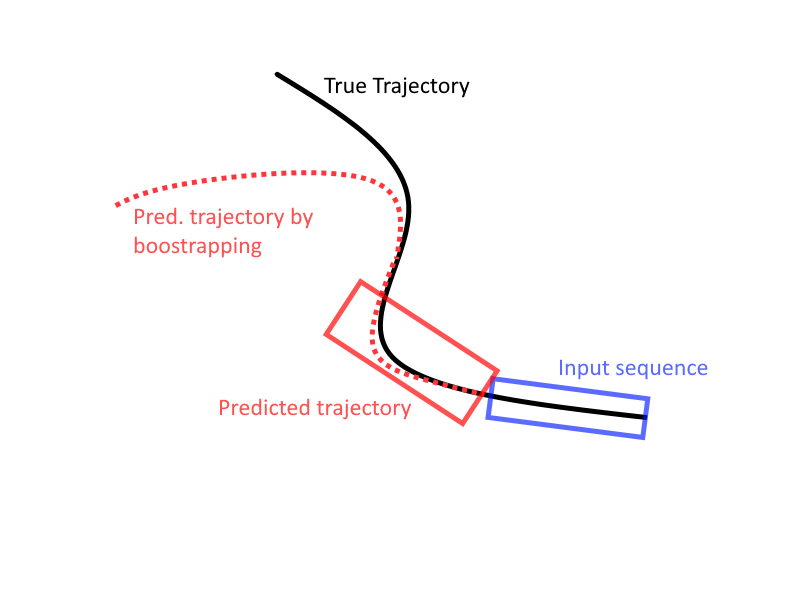
\includegraphics[width=0.75\textwidth]{images/LSTM_trajectory_window_example.png}
    \caption{Illustration of the accumulated prediction error by bootstrapping input sequences for an LSTM}
    \label{fig:lstm}
\end{figure}

\newpage
With the rise of deep reinforcement learning and its successful application in fields like robot control and autonomous system (\cite{s18092905, zare2021continuous, 9195789, martinsen2018curved}), the question comes to mind if this task can be formulated as a reinforcement learning problem as well. The idea behind using reinforcement learning is that training an agent to control an unmanned vessel results in a policy that learns end-to-end trajectories to get to a predefined destination. By replacing the simulated real-world environment with samples from normal vessel trajectories and tweaking the reward function, the assumption is that the agent learns to mimic normal vessel behaviour to eventually predict end-to-end trajectories.
\par
To give an example of what the agent should eventually learn, we illustrate two density maps of vessel trajectories generated by \cite{martinetraffic} for the year 2020:
\begin{figure}[H]
    \centering
    \begin{minipage}{.47\textwidth}
      \centering
      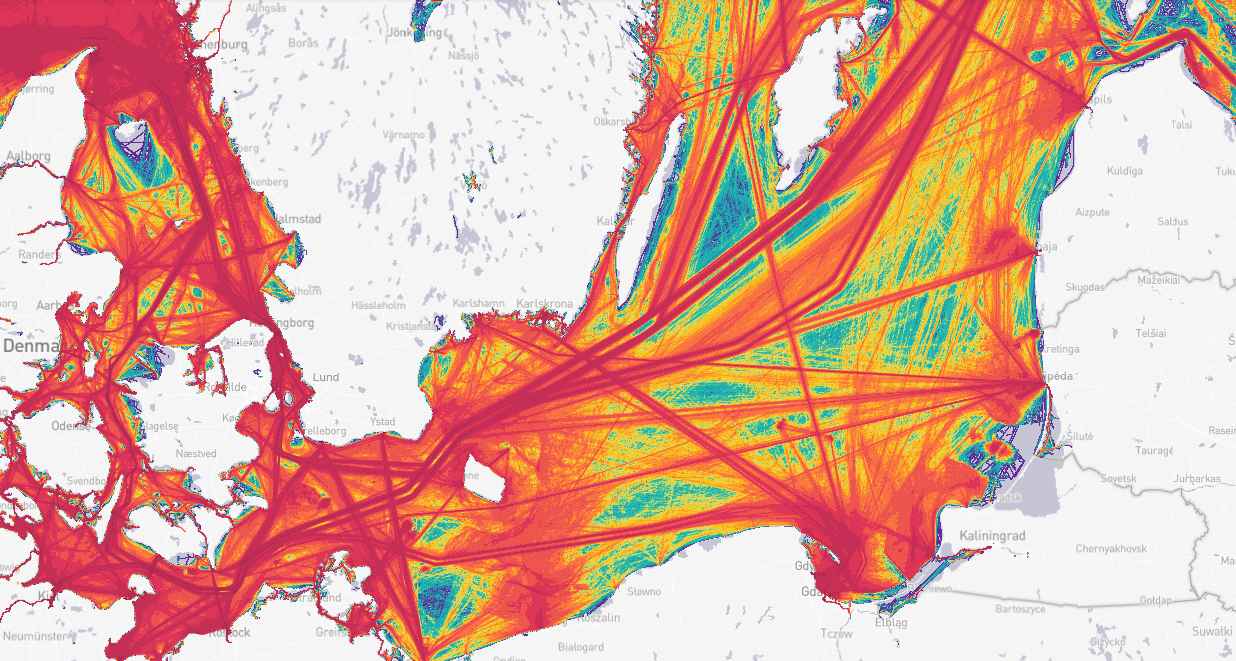
\includegraphics[width=\textwidth]{images/balticsea_density_routes.PNG}
      \captionof{figure}{Density map of vessel trajectories in the Baltic Sea}
      \label{fig:baltic}
    \end{minipage}
    \hspace{.05\textwidth}%
    \begin{minipage}{.47\textwidth}
        \centering
        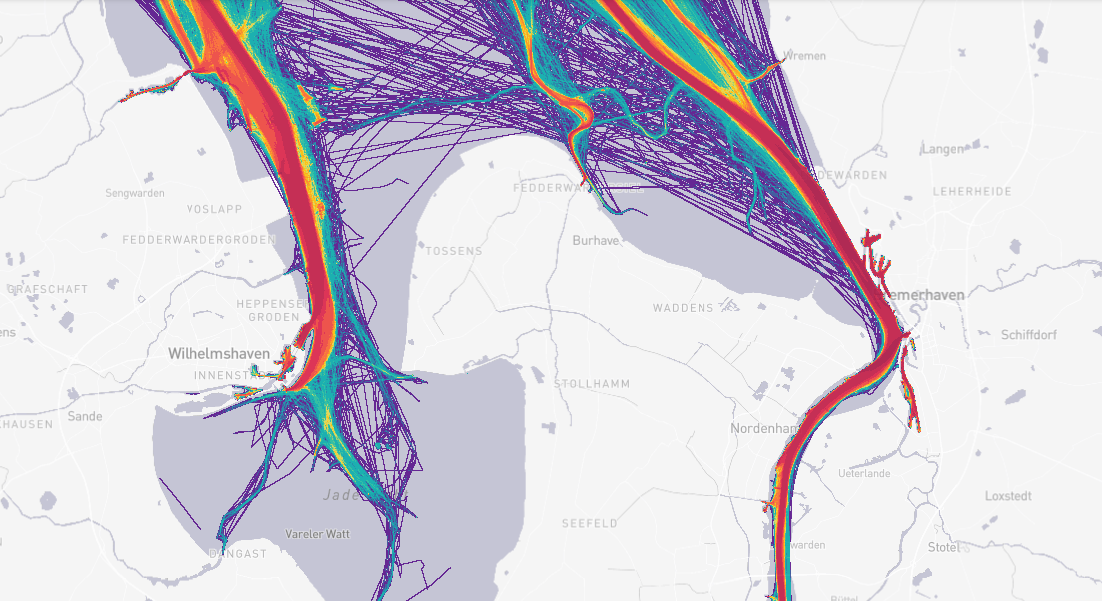
\includegraphics[width=\textwidth]{images/bhv_jadebusen_density_routes.PNG}
        \captionof{figure}{Density map of vessels near Bremerhaven and the Jadebusen}
        \label{fig:jadebusen}
      \end{minipage}
\end{figure}
Looking at figure \ref{fig:baltic}, we can discover the international shipping routes by following the red lines which indicate a high volume of vessel traffic. Furthermore, we notice certain points where the majority of ships choose to somewhat suddenly change their heading. It is up to the agent to learn exactly those specific patterns as in break points, entry angles to the ports, speed values and so on. 
\par
We know that this is not the classic operation area of reinforcement learning but this thesis tries to explore a new area of application by tweaking state representations and reward functions to make an agent learn to mimic normal behaviour in a way, so that the detection of anomalies is possible in a later stage.
\newpage
\section{Objective}
The overall objective is the implementation of a system based on a reinforcement learning algorithm that is able to predict vessel trajectories based on historical AIS data. The results are evaluated and then compared to those of the previous work done at the institute involving classic sequential models like RNNs and LSTMs.
\par
One intermediate goal is to get a big overview of related work in terms of the anomaly detection of vessels and the recent application of reinforcement learning, most importantly the ones regarding path planning. Another underlying objective is the build up of intimate knowledge of deep reinforcement learning methods, especially those which use the actor-critic architecture.
\par

\section{Methodology}
Five month is a short period of time for such a complex research project. Therefore we try to avoid pitfalls by taking into account the advice of our supervisors as well as a great experience report on short-term machine learning projects in context of a master thesis from \cite{tim2018}. He is an associate professor at the University College London and a scientist at the Facebook AI Research organization. The main advice he is giving to students is that they should start from  abstract and simplistic scenarios so it is easier to fully understand what is going on, to then have the ability to intervene and change things up under clear assumptions.
\par 
The planned sequence of tasks involve:
\begin{itemize}
    \item An in-depth literature review to discover similar works and recent trends
    \item The implementation of at least one deep reinforcement learning algorithm from scratch using PyTorch (most likely starting with DDPG)
    \item Designing a simple environment to show that reinforcement learning (RL) is indeed able to learn to reconstruct a family of curves (proof-of-work) 
    \item Applying the RL algorithm to the same learning setting (involving AIS data) of the previous approaches at the institute and compare results
    \item Tweaking of state representation and increase the number of AIS vessel trajectories
    \item (optional, plan B) The analysis of other methods such as offline RL and the usage of the transformer architecture as proposed by \cite{chen2021decision} 
\end{itemize}
\section{Related Work}
After a profound literature research, we can divide the related work into two sub categories. Those include the topics of building a framework for anomaly detection in the maritime domain and the general application of machine learning in path planning or prediction.

%different approaches to reinforcement learning such as inverse- and offline reinforcement learning and the ongoing work done in the field of deep reinforcement learning.
\par 
\paragraph{Anomaly detection of vessel behaviour}
Building a maritime awareness system that operates in near real time by processing huge amounts of data from all kinds of different sources (AIS, radar systems, satellites, etc.) is not a trivial task. The work of \cite{tsogas2019geospatial} presents a system architecture named Geospatial Complex Event Processing Service (TRITON) that is capable of handling large volumes of incoming events using ActiveMQ as message broker and PostgreSQL as database which is optimized for storing and querying geospatial information. By using the Event Processing Language (EPL), the service is also able to detect abnormal vessel behaviour. Though the set of specific rules (vessel entering, exiting, crossing, moving away or approaching areas) have to be defined by domain experts \cite[p.~4]{tsogas2019geospatial} which is a critical limitation of the detector. The authors themselves are thus mentioning the usage of reinforcement and unsupervised learning in future work \cite[p.~9]{tsogas2019geospatial}.
\par 
The general approach of using geospatial data like AIS to learn motion patterns, that are eventually used to predict vessel paths and detect anomalies, is not a novelty. Instead of employing hand crafted rules, the highly cited work by \cite{ristic2008statistical} uses historical AIS data to extract motion patterns to train an anomaly detector by applying statistical methods such as adaptive kernel density estimation and particle filters. A motion pattern in this connection is defined by kinematic information including ship location and velocity but also by at least one mandatory attribute information - the ship's origin - to distinguish between overlapping motion patterns \cite[p.~2]{ristic2008statistical}. This could be an interesting factor when designing a suitable state representation to fulfill the Markov property.
\par 
In a recent summary of the related literature, \cite{zhang2020analysis} analyze the research trends of vessel abnormal behavior detection of the past ten years. They found that earlier work concentrated on the detection of just abnormal tracking positions mainly based on statistical methods by almost exclusively using movement data (position, speed, heading) of the perspective of a single ship (pp.~47-48). In contrast, more recent approaches try to detect anomalies in specific situations by including contextual information such as meteorological data, the interaction between ships, the perception of ship motion status (identification of fishing operations, ship towing push or ship gathering) and video data \cite[p.~50]{zhang2020analysis}. The usage of non-kinematic features should therefore be deflected to eventually construct a sophisticated anomaly detector that  truly has a sense of situational awareness. In their work, \cite{zhang2020analysis} conclude that detectors of abnormal vessel behaviour face major problems, such as poor comprehensiveness (cannot specify abnormality type and degree), difficulties with huge amounts of data due to the complexity of their algorithms and high false alarm rates because of subjectively chosen thresholds (p.~52).
\par 
As mentioned in chapter \ref{chap:intro}, the term \anf{anomaly} can mean many things even in the conjunction of AIS data. Detecting abnormal vessel behaviour solely based on the trajectory is the main focus of this thesis but there are other types as well. \cite{singh2020effectiveness} who are colleagues at the sister institute in Neustrelitz, near Berlin, focus on malicious and intentional AIS on-off switching (OOS) anomalies. In their paper they compare the performance of various AI techniques including support vector machines, k-nearest neighbours, decision trees, artificial neural networks and naive Bayesian towards detecting the AIS
OOS anomalies using real historical AIS data (p.~1). The results (99,9\% accuracy when using an artificial neural network \cite[p.~7]{singh2020effectiveness}) suggest that this specific task can be labeled as solved. 


\paragraph{Path prediction}
To predict the trajectories of vessels, \cite{liu2019vessel} use support vector regression (SVR) in conjunction with an algorithm called ACDE for  parameter optimization. ACDE stands for \anf{differential evolution based on adaptive control parameters} and is an improved version of the differential evolution algorithm which tackles stochastic parallel optimization and is based on evolutionary ideas in form of genetic algorithms \cite[pp.~1-3]{thangaraj2009simple}. In their work, \cite{liu2019vessel} also present algorithms on how to extract single trajectories from the AIS data using the unique maritime mobile service identification (MMSI) numbers and how to clean, de-noise and normalize the AIS data (pp.~9-11). As multivariable input or in the context of reinforcement learning this can also be called \textit{state}, the authors of this paper are using unix timestamps, longitude, latitude, course and speed over ground of the ship (p.~11). We can redefined their input as state definition for a better overview, where $COG_t$ and $SOG_t$ are course and speed over ground respectively:
\begin{equation}
S_t = \{lon_t, lat_t, COG_t, SOG_t, Unix_t\}
\end{equation}
Four of those previous states plus the timestamp of the next moment $T_{t+1}$ will be the true input for two separate SVR models, one predicts the longitude $lon_{t+1}$ and the other predicts the latitude $lat_{t+1}$ for just one moment in advance \cite[p.~11]{liu2019vessel}. Predicting just the next timestamp in advance, this method might be not suitable in terms of forecasting a complete vessel trajectory because of the major concern that this model will accumulate error if a prediction output is used as input for a larger forecasting window.
\par
In a recent published paper, \cite{venskus2021unsupervised} tackle the exact same topic of this thesis, that is the prediction of vessel trajectories based on historical AIS data in an unsupervised manner. They use an LSTM autoencoder that learns to reconstruct vessel paths for the next $X$ timestamps (p.~724). Furthermore the authors utilize a method proposed by \cite{cruz2019} to eventually generate a prediction region that is learned by two supplementary LSTM autoencoders in addition to the  most like-hood forecast of the original autoencoder that learns single trajectories (p.~725). Predicting a potential region that vessels under normal behavior would navigate in, makes anomaly detection trivial by just checking if the prognosticated path is inside the region that is considered \anf{normal}. Nevertheless a major constraint of this method is the needed input sequence of past $X$ timestamps to start forecasting the next $X$ timestamps.
\par 
\cite{perera2012maritime} introduce a framework to monitor maritime traffic by constructing three modules. The first module consists of an artificial neural network that detects and tracks multiple vessels while the second and third modules are used to estimate the vessel states and forecast the navigational trajectory by using an extended Kalman filter \cite[p.~1]{perera2012maritime}. 
\par 
A complete different approach is presented by \cite{6198334} who take advantage of the genetic algorithm in conjunction with randomly generated Bezier curves to solve the path planning of  autonomous unmanned aerial vehicles (UAVs) in previously defined environments~(p.~1). Besides they achieve quasi-linear speedup in relation to the number of CPU cores by using a parallel programming paradigm called \anf{single-program,
multiple-data} (pp.~7-8). Although the authors themselves state that the planning takes 10 seconds while running on eight cores in parallel, they still make the conclusion that \anf{real-time path planning for UAVs is possible} \cite[p.~9]{6198334}. However, we see this computational cost as critical limitation of classic genetic algorithms in general. Even though vessel planning cuts one dimension as the prediction of UAVs paths takes place in a 3D domain, we still make the assumption that this approach is not suitable for future visions of calculating vessel paths of hundreds of ships in near real-time. 
\par 
Entering the field of deep reinforcement learning, we can notice that most works are related to the control or path planning of unmanned vehicles (land, water or air) without focusing specifically on anomaly detection but rather control. \cite{etemad2020using} and \cite{zare2021continuous} for example utilize the classic Floyd–Warshall algorithm as path-planner and apply deep Q-learning or Deep Deterministic Policy Gradient (DDPG) respectively to tackle obstacle avoidance for unmanned surface vehicle (USV). In this case, deep reinforcement learning is used to evaluate the current situation (local view) on the USV's path and makes short-term decisions to avoid collisions (p.~8).

\par
The usage of Deep RL not only as supportive mechanism for short-term decision making but rather as full control algorithm for intelligent vehicles is the main field of application for reinforcement in general and, 
as a consequence, is strongly present in the literature. \cite{wang2018reinforcement} for instance take advantage of DDPG to control an autonomous underwater vehicle (AUV) in an under-ice environment that eventually learns the long-term reward of reducing the field uncertainty and the AUV mobility cost (p.~17). Another example is the work of \cite{s18092905} whose agent represents a land vehicle. They extract an abstract model of the real environment to then teach the agent driving maneuvers like overtaking, following a curve, ramp driving as well as staying in lane (pp.~1,4). As the agent is trained by the DDPG algorithm, it implicitly learns to drive on or near the desired path. This is mainly accomplished by defining the desired path and using the difference between the current posture and the desired one as part of the reward signal \cite[p.~4]{s18092905}. After training the agent in the virtual environment, the authors transfer their model and their \anf{end-to-end trajectory planning} (p.~17) to a real world scenario by letting the agent control a self driving bus (pp.~18-19).
\par
Staying in the maritime domain, we can identify the inventiveness of crewless autonomous ship systems as the closest research topic to the one of this thesis. In this field, \cite{s20020426} present a paper that uses the actor-critic algorithm DDPG to select actions which navigate a vessel on the fastest way to the target destination while also taking into account ship encounters (pp.~13-14). The important parts of their path planning module are the environment and the reward function. For the environment they choose a combination of two components. The first one is the \anf{Ship Action Controller} which converts the model output to an actual action that the unmanned ship should take (p.~15). The second one is the so called \anf{Ship navigation information fusion module} which is able to receive data from GPS, AIS, depth sounder and anemometer to construct a state that holds information about the ship itself, obstacles and the target point (p.~10). The reward signals is built by transforming the crew's experience and the navigation rules defined by COLREGS \cite[]{COLREG} into navigation restriction areas \cite[p.~14]{s20020426}. Crossing a restricted area or colliding with an obstacles results in a negative reward. Additionally the inverse of the distance between the agent and the target point is also granted as reward signal \cite[p.~14]{s20020426}. The results displayed by the authors are promising as the agent not only learns to get to the destination on the shortest path while avoiding obstacles but also reacts and adopts to multiple ships on its path
\cite[pp.~21-26]{s20020426}.
\par 
Instead of learning online by interacting with an environment it is also possible to learn offline by using historical AIS data. This approach is followed by \cite{westerlund2021learning} who uses offline reinforcement learning. The goal of his master thesis is to make an agent (the vessel) learn to get to a destination based on previously sampled data from a simulator. The simulator outputs a series of AIS data points representing the taken vessel trajectories which is used as data set. Here, the state is defined by latitude, longitude, speed over ground, course over ground, and most importantly the rudder angle while the action space only consists of the heading the ship should have at the next timestamp \cite[pp.~30-33]{westerlund2021learning}. To fully build the necessary tuples that get fed into the replay buffer $(s_t, a_t, r_{t+1}, s_{t+1})$, the author calculates the reward based on the difference between the current position and the targeted one (p.~27). Although the presented results show that it would generally be possible to apply offline reinforcement learning to the path planning problem of vessels, the author himself states that performance is \anf{limited by the size and diversity of the dataset}(p.~40) as the generalization outside the trained area is deficient.
\par
The previously cited works are better categorized as \anf{path finders} which means that their reward function is built around finding the best or potential new route to a destination. This lies in the nature of reinforcement learning being mainly used in control problems that try to come up with a policy that has learned the underlying dynamics of an environment. Even if the training data is not sampled online but generated in the past (as in the work  from \cite{westerlund2021learning}), the reward function is still defining the semantic of the goal which is very different from the goal of learning representative trajectories for future anomaly detection. For this specific setting the term \anf{path follower} might be more fitting. We found a paper from \cite{martinsen2018curved} which focuses exactly on this topic of following of a predefined curved path by a vessel. In their work they use DDPG and a Gaussian reward function that is mainly built from a cross-track error which tells how far away the vessel is from the predefined path \cite[p.~3]{martinsen2018curved}. 
\newpage
\section{Timetable}
% Please add the following required packages to your document preamble:
% \usepackage{graphicx}
\begin{table}[H]
\centering
\resizebox{\textwidth}{!}{%
\begin{tabular}{|l|l|l|}
\hline
\textbf{Task}                                                                                                              & \textbf{Milestone}                 & \textbf{Done Until}   \\ \hline
Literature review                                                                                                          &                                    & \multicolumn{1}{c|}{} \\ \cline{1-1}
Write exposé                                                                                                               &                                    & \multicolumn{1}{c|}{} \\ \cline{1-1}
Register thesis                                                                                                            & Master's thesis registration       & 30.09                 \\ \hline
Implement DDPG from scratch                                                                                                &                                    &                       \\ \cline{1-1}
\begin{tabular}[c]{@{}l@{}}Apply algorithm to simplistic \\ environment\end{tabular}                                       &                                    &                       \\ \cline{1-1}
\begin{tabular}[c]{@{}l@{}}Detailed logging and behaviour\\ documentation\end{tabular}                                     &                                    &                       \\ \cline{1-1}
\begin{tabular}[c]{@{}l@{}}Write chapter about Actor-Critic\\ and DDPG algorithm\end{tabular}                              & Agent following a famliy of curves & 8.11                  \\ \hline
\begin{tabular}[c]{@{}l@{}}Reuse gym environment\\ for AIS trajectories\end{tabular}                                       &                                    &                       \\ \cline{1-1}
\begin{tabular}[c]{@{}l@{}}Make DDPG, TD3 and SAC\\ work for this learning setting\end{tabular}                            &                                    &                       \\ \cline{1-1}
\begin{tabular}[c]{@{}l@{}}Document and compare results\\ to past experience\end{tabular}                                  & Finished comparison to LSTM        & 13.12                 \\ \hline
\begin{tabular}[c]{@{}l@{}}Process AIS data and extract\\ trajectories\end{tabular}                                        &                                    &                       \\ \cline{1-1}
\begin{tabular}[c]{@{}l@{}}Tweak gym environment\\ for AIS trajectories\end{tabular}                                       &                                    &                       \\ \cline{1-1}
Test different approaches                                                                                                  & Agent performs in real-world data  & 17.01                 \\ \hline
\begin{tabular}[c]{@{}l@{}}Write chapters about learning setup,\\ hyperparameters, performance and\\ findings\end{tabular} &                                    &                       \\ \cline{1-1}
Write down conclusions                                                                                                     &                                    &                       \\ \cline{1-1}
Write introduction and motivation                                                                                          & Writing finished                   & 07.02                 \\ \hline
Visualize results                                                                                                          &                                    &                       \\ \cline{1-1}
Improve quality of texts                                                                                                   &                                    &                       \\ \cline{1-1}
Pass thesis to proofreaders                                                                                                & Thesis got submitted               & 14.02                 \\ \hline
\end{tabular}%
}
\label{tab:stoercodeDetailed}
\end{table}

\newpage
\bibliographystyle{apacite}
\bibliography{sources}
\newpage

%\appendix
%\section{Anhang}
\end{document}
